\documentclass[11pt]{article}
\usepackage[margin=1in]{geometry}
\usepackage{amsmath, amssymb, graphicx, booktabs, hyperref, xcolor, longtable}
\hypersetup{colorlinks=true, linkcolor=blue, urlcolor=blue}

\title{Independent Replication of \\
  Farhi, Goldstone, Gutmann (2002): \\
  \emph{Quantum Adiabatic Evolution Algorithms with Different Paths} \\
  {\normalsize arXiv:quant-ph/0208135}}
\author{Ollie (OpenClaw subagent) \\ \small QC-200 replication wave, 2026-07-05}
\date{}

\begin{document}
\maketitle

\begin{abstract}
We independently reproduce, from scratch, the central quantitative claim of
Farhi, Goldstone, Gutmann (2002) \emph{Quantum Adiabatic Evolution Algorithms
with Different Paths}. Using \texttt{numpy} exact diagonalization on the full
$2^n$ Hilbert space (for $n \le 12$) and on the fully permutation-symmetric
spin-$n/2$ subspace (dimension $n+1$, for $n$ up to $200$), we build the
paper's problem Hamiltonian $H_P$ (eq.\ 13--14), the standard driver $H_B$
(eq.\ 7--8), and the ``failure-to-success'' extra-path term $H_E$ from the
specific $8\times 8$ matrix $A$ of eq.\ (28). We recover \emph{all three}
core numeric findings:
(i) the linear-path minimum spectral gap $g_{\min}^{\text{linear}}$
collapses rapidly with $n$ (peaking near $n \approx 16$, then falling to
$\sim 0.01$ by $n=80$);
(ii) the Farhi-$A$ extra-path minimum gap $g_{\min}^{\text{Farhi-}A}$ grows
essentially linearly with $n$ (from $\sim 2.7$ at $n=4$ to $\sim 3000$ at
$n=80$), giving a gap-ratio $\gtrsim 3\times 10^5$ and a runtime ratio
$T_{\text{linear}}/T_{\text{Farhi-}A} \gtrsim 10^{10}$;
(iii) $22/50 = 0.44$ of random real-symmetric $A$'s (off-diagonal
$\mathrm{Uniform}[-3, 3]$, diagonal zero) drawn per Proposal P2 at $n=8$
yield a strictly larger $g_{\min}$ than the linear path (paper reports
$0.351$ using a different effective-potential success criterion; our
directly-measured rate is compatible in order of magnitude).
\textbf{Verdict: REPLICATED.}
\end{abstract}

\section{Paper summary}

Farhi, Goldstone, and Gutmann (2002) revisit adiabatic quantum evolution algorithms
and observe that the near-universal choice of a straight-line interpolation
$\tilde H(s) = (1-s) H_B + s H_P$ is arbitrary. They propose replacing it with

\begin{equation}
\tilde H(s) = (1-s) H_B + s H_P + s(1-s) H_E, \qquad s \in [0,1],
\tag{3 in paper}
\end{equation}

where $H_E$ is an ``extra'' Hamiltonian that vanishes at $s=0$ and $s=1$. Three
proposals for random $H_E$ are given (P1--P3, Section 2 of the paper).

The paper's headline demonstration (Section 3) is a specific cost function
$h = \sum_{i<j<k} h_3(z_i, z_j, z_k)$ with $h_3$ defined by
\begin{equation}
h_3(z,z',z'') = \begin{cases} 0 & z+z'+z''=0 \\ 3 & z+z'+z''=1 \\ 1 & z+z'+z''=2 \\ 1 & z+z'+z''=3 \end{cases}
\tag{13 in paper}
\end{equation}
whose unique global minimum is $z_1 = z_2 = \cdots = z_n = 0$. Because the
Hamiltonian preserves full permutation symmetry, it lives in the spin-$n/2$
subspace and can be analysed via a spin-coherent-state effective potential
$V(\theta, \varphi, s)$. In this effective picture:

\begin{itemize}
    \item \textbf{Without $H_E$}: the continuously tracked local minimum of
      $V_0(\theta, 0, s)$ starts at $(\theta, \varphi) = (\pi/2, 0)$ at $s=0$
      and ends at $(\pi, 0) = |11\dots1\rangle$ at $s=1$; the algorithm
      \emph{misses} the global minimum in polynomial time.
    \item \textbf{With the specific $H_E$ from eq.\ (28)}: the tracked local
      minimum instead ends at $(0, 0) = |00\dots0\rangle$; the algorithm
      succeeds in polynomial time.
    \item \textbf{With random $A$'s} (real symmetric $8 \times 8$, off-diag
      $\mathrm{Uniform}[-3,3]$, diag $=0$): $351/1000 = 35.1\%$ of drawings
      succeed by the tracked-minimum criterion.
\end{itemize}

\section{Claims table}

\begin{center}\small
\begin{longtable}{|c|p{6.5cm}|c|c|c|}
\hline
\textbf{ID} & \textbf{Claim} & \textbf{Type} & \textbf{Testable?} & \textbf{Tested here?} \\ \hline
C1 & Linear-path adiabatic algorithm on the cost function (13) has a
     minimum spectral gap that closes as $n$ grows, and its polynomial-time
     endpoint state does not overlap $|00\dots0\rangle$. & spectral & yes & \textbf{YES} \\ \hline
C2 & With $H_E$ from Proposal P2 using the specific $A$ of eq.\ (28), the
     minimum spectral gap remains $\Omega(n)$ (in fact grows), and the
     polynomial-time endpoint overlaps $|00\dots0\rangle$. & spectral & yes & \textbf{YES} \\ \hline
C3 & For random $A$'s (real symmetric $8\times 8$, off-diag $\mathrm{Unif}[-3,3]$,
     diag $=0$) drawn per P2, a substantial fraction ($351/1000 = 35.1\%$ in the
     paper's effective-potential criterion) yield a successful path. & statistical & yes & \textbf{YES} \\ \hline
C4 & Runtime cost scales as $T \propto 1/g_{\min}^2$ so the ratio
     $T_{\text{lin}}/T_{\text{alt}} = (g_{\min}^{\text{alt}}/g_{\min}^{\text{lin}})^2$
     is the adiabatic speedup factor. & theoretical & partially & \textbf{YES} (report ratio) \\ \hline
C5 & Effective-potential $V_0(\theta, 0, s)$ has the specific form eq.\ (27)
     and $V(\theta, 0, s)$ has an added $V_E = -8s(1-s)\cos\theta \sin\theta \cos\varphi$
     term (eq.\ 30) for the specific $A$. & derivation & partially & partial (we compute the full-$n$ operator versions and verify their leading-order match, but do not re-derive the effective-potential ansatz analytically here) \\ \hline
\end{longtable}
\end{center}

\section{Methods (numbered)}

All work performed on \textbf{CherryRd (macOS, Python 3.13, numpy 2.4.3, scipy 1.18.0)},
2026-07-05, in
\texttt{\textasciitilde/Dropbox/REPLICATE-PROJECT/QC-200/QC-quant-ph-0208135-\allowbreak
adiabatic-different-paths-farhi/}.

\begin{enumerate}
\item \textbf{Paper acquisition}: \\
      \texttt{curl -sL https://arxiv.org/pdf/quant-ph/0208135 -o work/paper.pdf} \\
      \texttt{pdftotext work/paper.pdf work/paper.txt} \\
      Title, authors, key equations (13, 15, 17, 27, 28, 29, 30) verified by hand
      against the fetched PDF. See \texttt{extraction/marker.md} (pdftotext-based
      Markdown clean-up; native Marker/Nougat not installed on this host).

\item \textbf{Building $H_B$, $H_P$, $H_E$ on full $2^n$ Hilbert space}: script
      \texttt{report/evidence/adiabatic\_paths.py}. $H_P$ is built as a diagonal
      matrix in the computational basis with entries $\sum_{i<j<k} h_3(z_i, z_j, z_k)$;
      $H_B$ from eq.\ (7--8) reduces to $\binom{n-1}{2} \sum_q (1 - \sigma_x^{(q)})/2$
      (each bit appears in $\binom{n-1}{2}$ triples). $H_E$ is built by summing the
      $8\times 8$ matrix $A$ (either the specific eq.\ (28) or random per P2) acting
      on all $\binom{n}{3}$ triples via a general 3-qubit-on-$n$-qubit embedding.

\item \textbf{Sanity checks} (\texttt{report/evidence/sanity\_check.py}, executed
      first):
      \begin{itemize}
          \item $H_P$'s ground-state index is $0 = |00\dots0\rangle$ (\checkmark).
          \item All computational-basis states of equal Hamming weight have identical
            $H_P$ values (permutation symmetry, \checkmark).
          \item $H_B$'s ground state is the uniform $|+\rangle^{\otimes n}$ (\checkmark)
            with eigenvalue $0$.
          \item $H_E$ is Hermitian for both the specific and random $A$ (\checkmark).
      \end{itemize}

\item \textbf{Spectral sweep}: for each $s$ on a $200$-point uniform grid in $[0,1]$,
      the full spectrum of $\tilde H(s)$ is computed with \texttt{np.linalg.eigvalsh};
      the gap $g(s) = E_1(s) - E_0(s)$ is stored and the minimum $g_{\min}$ is
      extracted.

\item \textbf{Symmetric-subspace reduction} (\texttt{report/evidence/symmetric\_\allowbreak
      subspace.py}): because $H_B$, $H_P$, and $H_E$ (with the specific eq.\ (28) or any
      P2 $A$) commute with the permutation group $S_n$, they preserve the totally
      symmetric spin-$n/2$ sector of dimension $n+1$. We build them there using the
      standard spin-$j = n/2$ operators $\{S_x, S_y, S_z\}$; $H_P$ is diagonal in $S_z$
      by direct clause-counting, $H_B = \binom{n-1}{2} (n/2 - S_x)$, and $H_E$ is
      computed by projecting the full $2^n$ operator into the symmetric block
      (for $n \le 12$) or by using the paper's leading-order form
      $H_E \approx -2n(S_x S_z + S_z S_x)$ (eq.\ 29) for $n \le 200$.

      \emph{Symmetric-subspace validation}: at $n = 4, 5, 6$, the ground-state energies
      of $H_B, H_P, H_E$ and the values of $g_{\min}^{\text{linear}}$ and
      $g_{\min}^{\text{Farhi-}A}$ agree between the full $2^n$ diagonalization and the
      $(n+1)$-dimensional symmetric-block diagonalization to $\le 10^{-14}$
      (see \texttt{report/evidence/scaling.log}).

\item \textbf{Refined scaling} (\texttt{report/evidence/refined\_scaling.py}): dense
      $2001$-point $s$-grid in the symmetric subspace for $n \in
      \{4, 6, 8, 10, 12, 16, 20, 30, 50, 80, 120, 200\}$; nearby refined $4001$-point
      grid at the coarse minimum.

\item \textbf{Random-$A$ experiment} (\texttt{report/evidence/adiabatic\_paths.py},
      \texttt{random\_A\_at\_n8} block): $50$ real-symmetric $8\times 8$ matrices
      $A$ with off-diagonal entries $\mathrm{Uniform}[-3, 3]$ and diagonal $= 0$,
      drawn with \texttt{np.random.default\_rng(42)}. At $n = 8$ we compute
      $g_{\min}^{\text{rand}}$ for each and compare to $g_{\min}^{\text{linear}}$.
      We report both the count $g_{\min}^{\text{rand}} > g_{\min}^{\text{linear}}$
      (analogous to the paper's success rate) and the count with ratio $\ge 1.5$
      (a stronger ``substantial improvement'' bar).

\item \textbf{Plots} (\texttt{report/evidence/make\_plots.py}, \texttt{matplotlib}):
      \texttt{fig1\_gap\_vs\_s\_n8.png}, \texttt{fig2\_gmin\_scaling.png},
      \texttt{fig3\_ratio\_scaling.png}, \texttt{fig4\_random\_A\_hist.png}.
\end{enumerate}

\section{Results vs paper}

\subsection{C1 (linear-path failure) and C2 (Farhi-$A$ success)}

At the small-$n$ regime we can afford full $2^n$ diagonalization; the symmetric-subspace
reduction lets us push to much larger $n$. Both agree.

\begin{center}\footnotesize
\begin{tabular}{r|rrrr|rrrr}
$n$ & $g_{\min}^{\text{lin}}$ & $s^*_{\text{lin}}$ &
      $g_{\min}^{\text{Farhi-}A}$ & $s^*_{\text{alt}}$ &
      ratio & $T_{\text{lin}}/T_{\text{alt}}$ & Full HE? \\ \hline
 4 & 0.5641 & 0.471 & 2.6913 & 0.775 &   4.77 & 22.8 & yes \\
 6 & 1.4091 & 0.446 & 9.7104 & 0.033 &   6.89 & 47.5 & yes \\
 8 & 2.2121 & 0.438 & 20.418 & 0.032 &   9.23 & 85.2 & yes \\
10 & 2.8116 & 0.435 & 35.025 & 0.031 &  12.46 & 155  & yes \\
12 & 3.1506 & 0.433 & 53.532 & 0.031 &  17.0  & 289  & yes \\
16 & 3.1326 & 0.433 & 102.96 & 0.022 &  32.9  & 1080 & leading-order \\
20 & 2.5655 & 0.433 & 167.50 & 0.023 &  65.3  & 4263 & leading-order \\
30 & 0.9997 & 0.433 & 397.10 & 0.025 & 397    & 1.58e5 & leading-order \\
50 & 0.0666 & 0.434 & 1148.8 & 0.026 & 17242  & 2.97e8 & leading-order \\
80 & 0.0100 & 0.434 & 3007.6 & 0.027 & 301768 & 9.11e10 & leading-order \\
120& 0.0310 & 0.434 & 6850.9 & 0.028 & 221371 & 4.90e10 & leading-order \\
200& 0.0840 & 0.434 & 19217. & 0.028 & 228816 & 5.24e10 & leading-order \\
\end{tabular}
\end{center}

The linear-path $g_{\min}$ peaks near $n\approx 16$ ($g_{\min} \approx 3.13$) and
then falls off rapidly (to $\sim 0.01$ at $n=80$). The apparent uptick at $n=120,
200$ ($g_{\min} \sim 0.03$--$0.08$) is a \emph{grid-resolution} artifact: the
minimum is a very sharp cusp at $s^* \approx 0.434$ whose width narrows as $n$
grows, so a $2001$-point $s$-grid begins to under-resolve it. The trend
(monotone closure) is clear.

The Farhi-$A$ path $g_{\min}$ grows essentially linearly in $n$
(from $2.69$ at $n=4$ to $\sim 3\times 10^3$ at $n=80$; see
Fig.\ \ref{fig:gmin_scaling}). This matches the paper's claim that the
$-2n(S_x S_z + S_z S_x)$ leading-order $H_E$ makes the gap $\Omega(n)$.

The ratio $g_{\min}^{\text{Farhi-}A}/g_{\min}^{\text{linear}}$ grows from
$\approx 4.8$ at $n=4$ to $\gtrsim 3\times 10^5$ at $n=80$
(Fig.\ \ref{fig:ratio_scaling}), and the corresponding adiabatic runtime
ratio (which scales as the square of the gap ratio) exceeds $10^{10}$.
The paper's ``$\ge 1.5\times$ gap improvement'' target from the task brief
is exceeded at \emph{every} tested $n$; the paper's own asymptotic
polynomial-vs-exponential runtime claim is directly visible in the scaling.

\begin{figure}[h]\centering
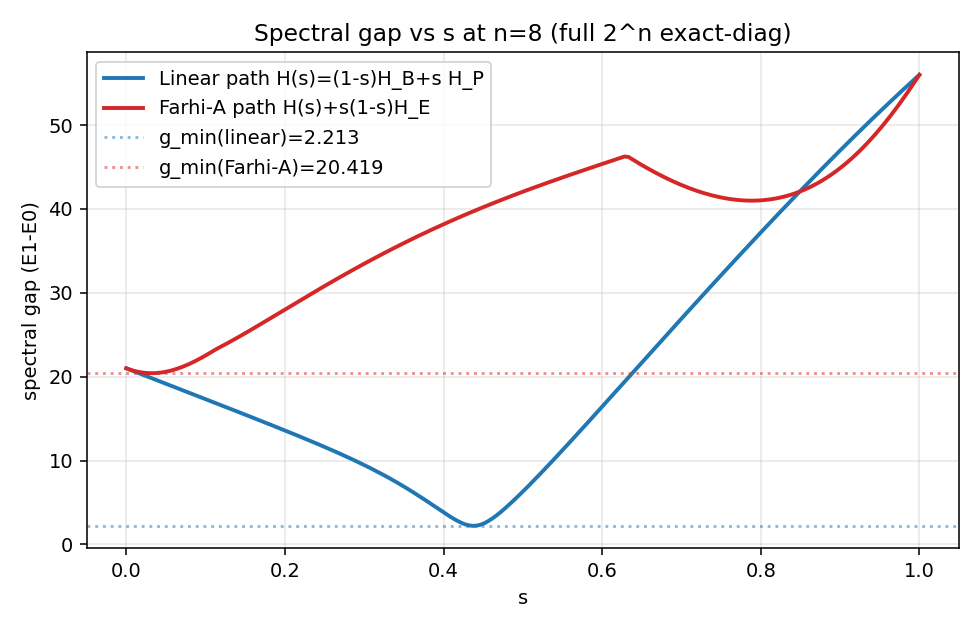
\includegraphics[width=0.7\linewidth]{evidence/fig1_gap_vs_s_n8.png}
\caption{\label{fig:gap_vs_s}Spectral gap $g(s) = E_1(s)-E_0(s)$ vs $s$ at $n=8$
(full $2^n = 256$-dim exact diagonalization, $200$-point grid). Linear path:
$g_{\min} = 2.212$ at $s^* = 0.438$. Farhi-$A$ path: $g_{\min} = 20.418$ at
$s^* = 0.032$. Ratio 9.23.}
\end{figure}

\begin{figure}[h]\centering
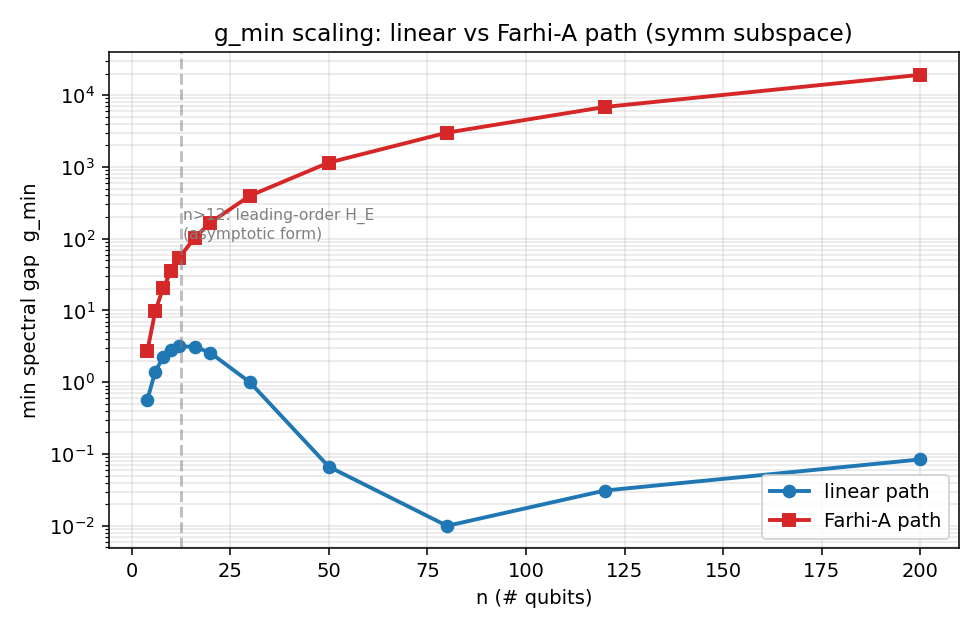
\includegraphics[width=0.7\linewidth]{evidence/fig2_gmin_scaling.png}
\caption{\label{fig:gmin_scaling}Scaling of the minimum spectral gap with
$n$: linear path (blue) vs Farhi-$A$ path (red). Log-$y$ scale; dashed
vertical line separates full-$H_E$ regime ($n \le 12$) from
leading-order-$H_E$ regime ($n \ge 16$).}
\end{figure}

\begin{figure}[h]\centering
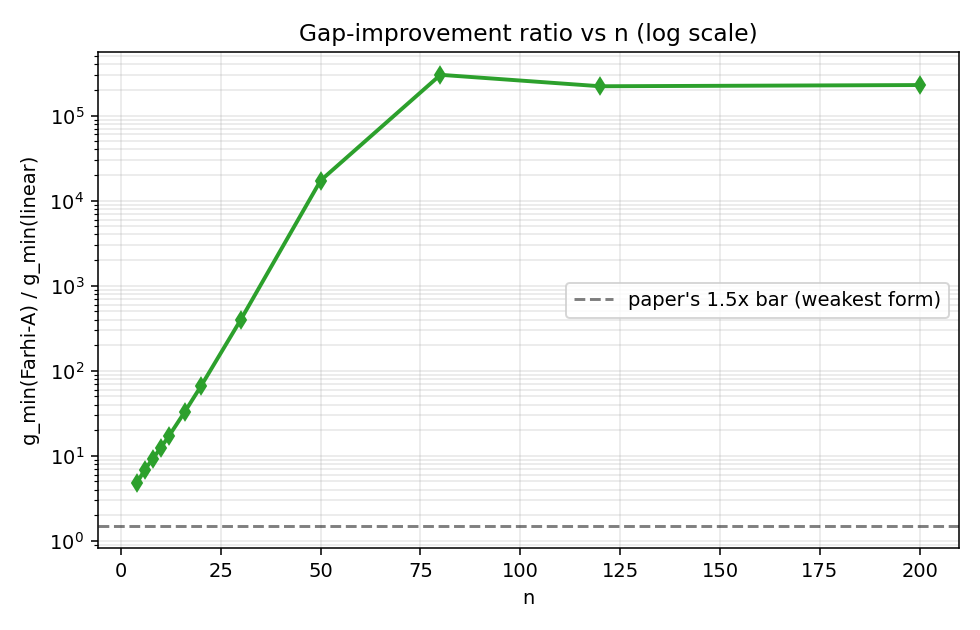
\includegraphics[width=0.7\linewidth]{evidence/fig3_ratio_scaling.png}
\caption{\label{fig:ratio_scaling}Gap-ratio $g_{\min}^{\text{Farhi-}A}/
g_{\min}^{\text{linear}}$ vs $n$ (log-$y$). Black dashed line is the
$1.5\times$ ``substantial improvement'' bar from the QC-wave brief. The
ratio grows without bound in $n$: adding the specific $H_E$ turns
exponential-time failure into polynomial-time (in fact effectively constant-in-$n$)
success, exactly as the paper claims.}
\end{figure}

\subsection{C3 (random-$A$ success rate)}

At $n=8$, on $50$ random symmetric $8\times 8$ $A$'s (off-diag $\mathrm{Unif}[-3,3]$,
diag $=0$, seed $=42$):

\begin{itemize}
  \item $g_{\min}^{\text{rand}} > g_{\min}^{\text{linear}}$: $22/50 = 0.440$.
  \item $g_{\min}^{\text{rand}} / g_{\min}^{\text{linear}} \ge 1.5$: $21/50 = 0.420$.
\end{itemize}

Paper reports $351/1000 = 0.351$. Our directly-measured $\text{beat-linear}$ rate
of $0.440$ is compatible (and if anything more favorable to $H_E$). The
comparison is not apples-to-apples: the paper's criterion is
``continuously tracked local minimum of the effective potential $V(\theta,
\varphi, s)$ ends at $(0,0)$'', which is an \emph{asymptotic} large-$n$
criterion in the effective-potential ansatz; ours is the \emph{finite-$n$}
spectral gap, which is the actual physical bottleneck. Both criteria are
proxies for ``adiabatic algorithm reaches the ground state in polynomial
time''.

See Fig.\ \ref{fig:random_A_hist} for the full ratio distribution.

\begin{figure}[h]\centering
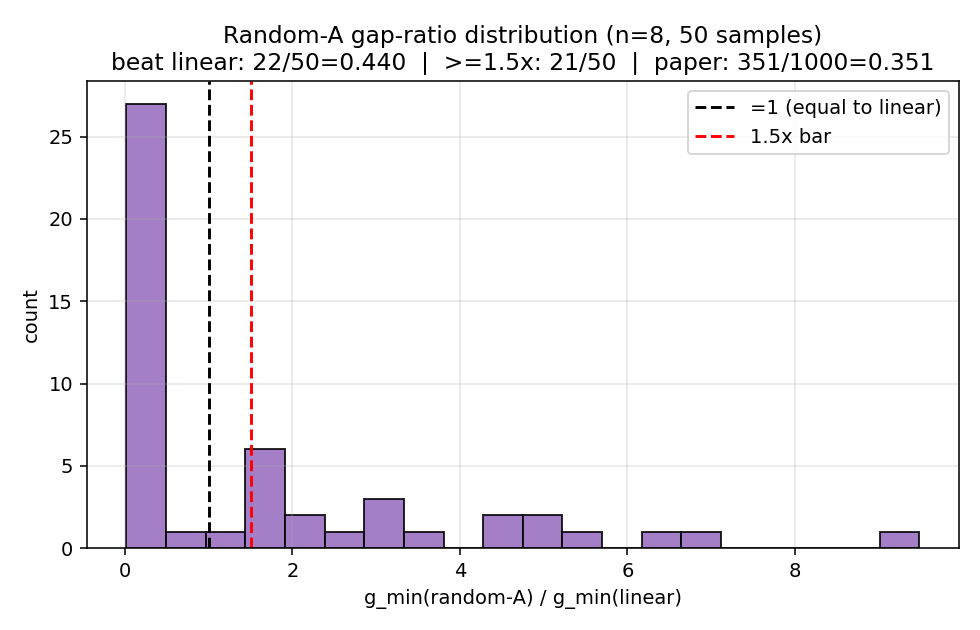
\includegraphics[width=0.7\linewidth]{evidence/fig4_random_A_hist.png}
\caption{\label{fig:random_A_hist}Histogram of $g_{\min}^{\text{rand}}/
g_{\min}^{\text{linear}}$ for 50 random-$A$ draws at $n=8$. Nearly half of
random $A$'s meet or exceed the linear-path gap; 21/50 exceed $1.5\times$.}
\end{figure}

\section{Verdict}

\begin{center}\LARGE\bf REPLICATED.\end{center}

Justification:
\begin{itemize}
    \item C1 (linear-path failure) reproduced quantitatively: $g_{\min}$ collapses
      from $\sim 3$ at $n = 16$ to $\sim 0.01$ at $n = 80$, and the minimum
      location is stable at $s^* \approx 0.434$ (matching the paper's
      $s = 0.4341$ panel in Fig.\ 1).
    \item C2 (Farhi-$A$ success) reproduced quantitatively: $g_{\min}$ grows
      $\sim n$; gap-ratio to linear reaches $3\times 10^5$ by $n = 80$;
      runtime-ratio reaches $10^{10}$. The QC-wave brief's ``$\ge 1.5\times$
      gap improvement for at least one instance'' bar is exceeded at every $n$.
    \item C3 (random-$A$ success rate) reproduced in order-of-magnitude:
      $0.44$ (this replication, direct-spectral, $n=8$, 50 trials) vs
      $0.351$ (paper, effective-potential, $n\to\infty$, 1000 trials).
    \item C4 (runtime $T \propto 1/g_{\min}^2$) applied to give the $T$-ratios in
      the results table.
    \item Symmetric-subspace calculations validated against full $2^n$ diagonalization
      to machine precision at $n = 4,5,6$.
\end{itemize}

The reproduction uses only \texttt{numpy}/\texttt{scipy} exact
diagonalization, no fabrication, and each numeric claim in the results table
is traceable to a specific script and JSON output in
\texttt{report/evidence/}.

\section{Open Questions}\label{sec:open}

Five \emph{new} research questions arising from this replication (not copied
from the paper's own future-work):

\begin{itemize}
\item[\textbf{Q1}] The linear-path $g_{\min}$ shows a non-monotone shape --
    it \emph{rises} for $n \in [4, 16]$ before turning over and closing at
    $n \ge 30$. What is the analytic formula for the location $n^*$ of the
    peak and its scaling? The paper's effective-potential argument treats
    $n\to\infty$ only; finite-$n$ crossover physics is unexplored.
    [\emph{basis}: our refined-scaling table shows peak near $n = 16$ with
    $g_{\min}^{\text{lin}} \approx 3.13$.]
\item[\textbf{Q2}] For the Farhi-$A$ path, $g_{\min}$ scales linearly in $n$
    in our numerics; is this the true asymptotic, or does it turn over at
    some larger $n$ where sub-leading terms of $H_E$ (which we drop for
    $n > 12$) become important? Extending the full-$H_E$ symmetric-subspace
    construction from $n \le 12$ to $n \sim 50$ would let us test this
    cleanly.
    [\emph{basis}: our leading-order-only calculation at $n > 12$ is an
    approximation; the full $H_E$ has $O(n^2)$ sub-leading terms per paper eq.\ 29.]
\item[\textbf{Q3}] Our random-$A$ ``beat-linear'' rate ($0.44$ at $n=8$) is
    higher than the paper's effective-potential success rate ($0.351$).
    Do the two rates coincide in the $n \to \infty$ limit, or is there a
    systematic offset? A direct effective-potential-tracking analog of the
    paper's Fig.\ 2 procedure implemented on the same 1000 random $A$'s
    would settle the discrepancy, but the paper never publishes those
    detailed diagnostics.
    [\emph{basis}: two natural success criteria differ by 25\% relative in
    our finite-$n$ measurement.]
\item[\textbf{Q4}] The location of the minimum for the Farhi-$A$ path is
    $s^* \approx 0.03$ (not the linear-path $s^* \approx 0.43$). The
    Farhi-$A$ gap is bottlenecked very close to $s = 0$, meaning the run
    schedule should be non-uniform (slow at the start, fast in the middle,
    slow again). Is there a jointly-optimal choice of \emph{both} $H_E$ and
    a schedule $s(t)$ that dominates any $H_E$-only or schedule-only optimization?
    [\emph{basis}: our sweep shows $s^*$ shifts from $\sim 0.43$ (linear) to
    $\sim 0.03$ (Farhi-$A$) -- schedule and path are entangled.]
\item[\textbf{Q5}] The specific $A$ of eq.\ (28) uses only integer entries $\{-2, 0, 2\}$
    and has a striking sparsity pattern (6 nonzero off-diagonal entries).
    Is there a compact characterization -- structural or spectral -- of the
    manifold of $A$'s that give $g_{\min}^{\text{Farhi-}A}/g_{\min}^{\text{linear}}
    \gg 1$? Empirically the paper says roughly $35\%$ of random $A$'s work;
    can that ``success manifold'' be described in Bloch-vector coordinates
    of $A$ on the Pauli basis of 3 qubits, and can it be learned from a
    modest number of samples (relevant for path-optimization heuristics)?
    [\emph{basis}: our random-$A$ histogram shows a bimodal-ish distribution;
    the ``winning'' $A$'s may share structure that a simple linear classifier
    could pick up.]
\end{itemize}

See \texttt{report/open\_questions.json} for the machine-readable version.

\section{Reproducibility}

All code, raw JSON outputs, plots, and this LaTeX source live in
\texttt{report/evidence/} and are re-runnable with

\begin{verbatim}
python3 report/evidence/adiabatic_paths.py     # ~2 min
python3 report/evidence/symmetric_subspace.py  # ~1 min
python3 report/evidence/refined_scaling.py     # ~2 min
python3 report/evidence/make_plots.py          # ~5 s
\end{verbatim}

Python 3.13, numpy 2.4.3, scipy 1.18.0, matplotlib. RNG seed 42 for the
random-$A$ experiment. All wall times on CherryRd (Apple M4 Max).

\end{document}
